% Document type, global settings, and packages

\documentclass[12pt, openany]{report}   %12 point font for Times New Roman
\usepackage{graphicx}  %for images and plots
\usepackage[letterpaper, left=1in, right=1in, top=1in, bottom=1in]{geometry}
\usepackage{setspace}  %use this package to set linespacing as desired
\usepackage{times}  %set Times New Roman as the font
\usepackage[explicit]{titlesec}  %title control and formatting
\usepackage[titles]{tocloft}  %table of contents control and formatting
\usepackage[backend=bibtex, sorting=none, bibstyle=ieee]{biblatex}  %reference manager
\usepackage{appendix}  %for appendices
\usepackage{rotating}  %for rotated, landscape images
\usepackage[normalem]{ulem}  %for underlined section titles
\usepackage{textcomp} % for text symbols such as copyright etc. 
\usepackage{indentfirst} % To indent the first line of every paragraph
\usepackage{booktabs,array,arydshln} %for better table formatting. 
\usepackage{amsmath} %for formula formatting
\usepackage[T1]{fontenc} % improved font encoding
\usepackage[utf8]{inputenc} % for better handling of non-ASCII characters
%\usepackage{newtxtext} % font choice
\usepackage{newtxmath} 
%\usepackage{lmodern} % font choice 
%\usepackage[bookmarks=true, hidelinks]{hyperref}
\usepackage[hidelinks]{hyperref}
\usepackage{datetime}
%\usepackage{lastpage}  % Add the lastpage package
\usepackage{refcount}
%\usepackage[acronym]{glossaries}
\usepackage[acronym,nomain,nonumberlist]{glossaries}
\usepackage{acronym}
\usepackage[font=bf]{caption}

\makeglossaries

% List acronyms you would like to have appear in the List of Abbreviations. 

% Each acronym is in the format \newacronym{tag}{acronym}{long}

% The "tag" field is used when defining the acronym in the main text. The "acronym" field contains the abbreviated form, and the "log" field contains the unabbreviated definition.

% Note: in order for the acronym to appear in the List of Acronyms, it must be tagged in the main text.

% To tag the acronym in the main text, you can write something like:  \acrlong{dna} (abbreviated \acrshort{dna}) is the molecule that carries the genetic information for the development and functioning of an organism.

\newacronym{dna}{DNA}{Deoxyribonucleic acid}

 %glossary terms, make glossary

% Bibliography
%Add your bibliography file here
\bibliography{references}

% prevent certain fields in references from printing in bibliography
\AtEveryBibitem{\clearfield{issn}}
\AtEveryBibitem{\clearlist{issn}}

\AtEveryBibitem{\clearfield{language}}
\AtEveryBibitem{\clearlist{language}}

\AtEveryBibitem{\clearfield{doi}}
\AtEveryBibitem{\clearlist{doi}}

\AtEveryBibitem{\clearfield{url}}
\AtEveryBibitem{\clearlist{url}}

\AtEveryBibitem{%
  \ifentrytype{online}
    {}
    {\clearfield{urlyear}\clearfield{urlmonth}\clearfield{urlday}}}


% Start of Dissertation Document

\begin{document}
\doublespacing  %set line spacing to double by default through out the document. This can be overwritten when necessary

% Title Page (No page number)
\pagenumbering{gobble}
%This is the tile page of your dissertation
%Please type below title of your dissertation and your name
%change the year if neccessary
\newdateformat{monthyeardate}{%
\monthname[\THEMONTH] \THEYEAR}
  
\begin{titlepage}
\begin{center}

\begin{singlespacing}
\vspace*{2\baselineskip}

\includegraphics[width = 1.75 in]{figures/Seal-blue.png}\\
\vspace*{5\baselineskip}

TITLE HERE\\ % UPPER CASE

\vspace{8\baselineskip}
A Thesis Presented to the Faculty of\\
The Rockefeller University\\
in Partial Fulfillment of the Requirements for\\
the degree of Doctor of Philosophy\\
\vspace{8\baselineskip}
by\\
Student Name\\ % Fill in your name here
Month and Year of degree conferral (ex: May 2023) % 
\vspace{3\baselineskip}
\vfill


\end{singlespacing}

\end{center}
\end{titlepage}




% Copyright  Page (No page number)
\pagenumbering{gobble}


%\begin{titlepage}
\begin{singlespacing}
\begin{center}

\vspace*{40\baselineskip}

\textcopyright \, by Student Name \the\year\\ % Fill in your name here.
\vspace{\baselineskip}	

\end{center}
\vfill

\end{singlespacing}
%\end{titlepage}


% Abstract (No page number)
\pagenumbering{gobble}
%Abstract Page
%\begin{titlepage}
\begin{center}
\thispagestyle{empty}

TITLE 

Student Name\\
The Rockefeller University \the\year
\end{center}
\begin{flushleft}
\hspace{10mm}
\textbf{(Insert abstract here, about 1.5 pages long)}

Lorem ipsum dolor sit amet, consectetur adipiscing elit. Sed consequat mollis urna id rhoncus. Fusce a faucibus nibh. Vivamus porta aliquet metus, efficitur posuere lectus dignissim at. Duis scelerisque sapien non volutpat pellentesque. Vivamus ullamcorper nec sapien et suscipit. Vestibulum tristique egestas lectus, id porta urna cursus in. Suspendisse ut ipsum libero. Proin quis blandit purus. Etiam blandit lacinia placerat.

Maecenas quis aliquet dui, eget cursus dui. Duis facilisis mauris eu urna iaculis finibus. Morbi ex tellus, vulputate sit amet lobortis fermentum, vulputate sit amet diam. Sed facilisis est id dictum volutpat. Pellentesque tempus lacus sit amet sem mattis molestie. Mauris id convallis mauris. Etiam ullamcorper finibus elit.

Donec lacinia pulvinar nibh et pretium. Suspendisse at rutrum quam. Phasellus blandit non eros non bibendum. Cras vitae gravida enim. Aenean nec est odio. Sed aliquet ante vitae nulla efficitur, ut hendrerit massa dictum. Sed vitae facilisis urna. Cras diam sem, pulvinar non ultrices at, molestie id nunc. Morbi rhoncus in leo quis eleifend. Donec eget est id quam aliquet imperdiet. Cras gravida nisi in nunc interdum, vitae hendrerit tortor ultricies. Morbi ut metus laoreet, consectetur risus a, finibus libero. Nunc iaculis urna metus, vel vehicula tellus consequat non. Donec at magna risus. Vivamus vitae interdum diam.

Nam et erat eros. Cras sed laoreet nulla. Curabitur malesuada metus non metus ultrices vehicula. Nullam sit amet urna neque. Cras consectetur libero libero, sit amet pulvinar risus commodo at. Phasellus vulputate vulputate ex, id condimentum est eleifend ac. Morbi convallis sed lacus non placerat. Nullam eros metus, tincidunt sit amet pellentesque eget, egestas eu dolor.

In vitae convallis tellus, vel cursus magna. Integer vulputate nulla eget lorem tempus gravida. Etiam finibus, orci ac lobortis laoreet, sem magna elementum dui, ut varius lacus massa ut libero. Nam pretium, nisl sit amet elementum semper, nisl arcu congue arcu, nec fermentum dolor neque sit amet nibh. Suspendisse vitae odio a metus tempus dapibus malesuada et lectus. Morbi massa augue, vulputate id purus eget, aliquam auctor ipsum. Aenean justo leo, suscipit posuere tincidunt in, ornare at urna. Donec tempus id sapien nec viverra.

Lorem ipsum dolor sit amet, consectetur adipiscing elit. Sed consequat mollis urna id rhoncus. Fusce a faucibus nibh. Vivamus porta aliquet metus, efficitur posuere lectus dignissim at. Duis scelerisque sapien non volutpat pellentesque. Vivamus ullamcorper nec sapien et suscipit. Vestibulum tristique egestas lectus, id porta urna cursus in. Suspendisse ut ipsum libero. Proin quis blandit purus. Etiam blandit lacinia placerat.

Maecenas quis aliquet dui, eget cursus dui. Duis facilisis mauris eu urna iaculis finibus. Morbi ex tellus, vulputate sit amet lobortis fermentum, vulputate sit amet diam. Sed facilisis est id dictum volutpat. Pellentesque tempus lacus sit amet sem mattis molestie. Mauris id convallis mauris. Etiam ullamcorper finibus elit.

Donec lacinia pulvinar nibh et pretium. Suspendisse at rutrum quam. Phasellus blandit non eros non bibendum. Cras vitae gravida enim. Aenean nec est odio. Sed aliquet ante vitae nulla efficitur, ut hendrerit massa dictum. Sed vitae facilisis urna. Cras diam sem, pulvinar non ultrices at, molestie id nunc. Morbi rhoncus in leo quis eleifend. Donec eget est id quam aliquet imperdiet. Cras gravida nisi in nunc interdum, vitae hendrerit tortor ultricies. Morbi ut metus laoreet, consectetur risus a, finibus libero. Nunc iaculis urna metus, vel vehicula tellus consequat non. Donec at magna risus. Vivamus vitae interdum diam.

\end{flushleft}
\vspace*{\fill}
\pagenumbering{gobble}
%\end{titlepage}


% Dedication
%\phantomsection
\clearpage
\pagenumbering{roman}
\setcounter{page}{3}
\addcontentsline{toc}{chapter}{Dedication}
%Dedication page. 
%This page is optional


\topskip0pt
\vspace*{\fill}
\begin{flushleft}
\textit{Type your dedication here. This page is optional.}
\end{flushleft}
\vspace*{\fill}
\clearpage
%\pagenumbering{gobble}  %remove page number on summary page




% Acknowledgments
\phantomsection
\addcontentsline{toc}{chapter}{Acknowledgments}
%ACKNOWLEDGEMENTS page. 
%This page is optional

%\clearpage
\begin{center}

%\vspace*{5\baselineskip}
\textbf{\large Acknowledgements}
\end{center}


\begin{flushleft}
\hspace{10mm}Insert your acknowledgments text here. This page is optional, you may delete it if not needed. 

Lorem ipsum dolor sit amet, consectetur adipiscing elit. Sed consequat mollis urna id rhoncus. Fusce a faucibus nibh. Vivamus porta aliquet metus, efficitur posuere lectus dignissim at. Duis scelerisque sapien non volutpat pellentesque. Vivamus ullamcorper nec sapien et suscipit. Vestibulum tristique egestas lectus, id porta urna cursus in. Suspendisse ut ipsum libero. Proin quis blandit purus. Etiam blandit lacinia placerat.

Maecenas quis aliquet dui, eget cursus dui. Duis facilisis mauris eu urna iaculis finibus. Morbi ex tellus, vulputate sit amet lobortis fermentum, vulputate sit amet diam. Sed facilisis est id dictum volutpat. Pellentesque tempus lacus sit amet sem mattis molestie. Mauris id convallis mauris. Etiam ullamcorper finibus elit.

Donec lacinia pulvinar nibh et pretium. Suspendisse at rutrum quam. Phasellus blandit non eros non bibendum. Cras vitae gravida enim. Aenean nec est odio. Sed aliquet ante vitae nulla efficitur, ut hendrerit massa dictum. Sed vitae facilisis urna. Cras diam sem, pulvinar non ultrices at, molestie id nunc. Morbi rhoncus in leo quis eleifend. Donec eget est id quam aliquet imperdiet. Cras gravida nisi in nunc interdum, vitae hendrerit tortor ultricies. Morbi ut metus laoreet, consectetur risus a, finibus libero. Nunc iaculis urna metus, vel vehicula tellus consequat non. Donec at magna risus. Vivamus vitae interdum diam.

Nam et erat eros. Cras sed laoreet nulla. Curabitur malesuada metus non metus ultrices vehicula. Nullam sit amet urna neque. Cras consectetur libero libero, sit amet pulvinar risus commodo at. Phasellus vulputate vulputate ex, id condimentum est eleifend ac. Morbi convallis sed lacus non placerat. Nullam eros metus, tincidunt sit amet pellentesque eget, egestas eu dolor.

In vitae convallis tellus, vel cursus magna. Integer vulputate nulla eget lorem tempus gravida. Etiam finibus, orci ac lobortis laoreet, sem magna elementum dui, ut varius lacus massa ut libero. Nam pretium, nisl sit amet elementum semper, nisl arcu congue arcu, nec fermentum dolor neque sit amet nibh. Suspendisse vitae odio a metus tempus dapibus malesuada et lectus. Morbi massa augue, vulputate id purus eget, aliquam auctor ipsum. Aenean justo leo, suscipit posuere tincidunt in, ornare at urna. Donec tempus id sapien nec viverra.
\end{flushleft}
%\clearpage

%\pagenumbering{gobble}  %remove page number on summary page





% Table of Contents
%\currentpdfbookmark{Table of Contents}{TOC}
% Format for Table of Contents
\renewcommand{\cftchapdotsep}{\cftdotsep}  %add dot separators
\renewcommand{\cftchapfont}{\normalfont}  %set title font weight that shows up on TOC
\renewcommand{\cftchappagefont}{}  %set page number font-weight
\renewcommand{\cftchappresnum}{Chapter }
\renewcommand{\cftchapaftersnum}{:}
\renewcommand{\cftchapnumwidth}{6em}
\renewcommand{\cftchapafterpnum}{\vskip\baselineskip} %set correct spacing for entries in single space environment
\renewcommand{\cftsecafterpnum}{\vskip\baselineskip}  %set correct spacing for entries in single space environment
\renewcommand{\cftsubsecafterpnum}{\vskip\baselineskip} %set correct spacing for entries in single space environment
\renewcommand{\cftsubsubsecafterpnum}{\vskip\baselineskip} %set correct spacing for entries in single space environment

%format title font size and position (this also applies to list of figures and list of tables)
\titleformat{\chapter}[display]
{\normalfont\bfseries\filcenter}{\chaptertitlename\ \thechapter}{0pt}{\large{#1}}

\renewcommand\contentsname{Table of Contents}
\begin{singlespace}
\tableofcontents
\setlength{\cftparskip}{\baselineskip}
\newpage
\phantomsection
\addcontentsline{toc}{chapter}{List of Figures}
\listoffigures
\newpage
\phantomsection
\addcontentsline{toc}{chapter}{List of Tables}
\listoftables
\newpage
\phantomsection
\addcontentsline{toc}{chapter}{List of Abbreviations}
%\printglossary[type=\acronymtype, title=List of Abbreviations, toctitle=List of Abbreviations]
\clearpage\begingroup\let\newpage\relax\printglossary[title=List of Abbreviations]\endgroup
\end{singlespace}
%%%%%%%
%	            %
% Chapters   %
%                   %
%%%%%%%

% General formatting for chapters, appendix, etc. 


% reset page numbering for rest of document 
\newpage
%\setcounter{page}{1} 


% Adjust chapter title formatting
\titleformat{\chapter}[display]
{\normalfont\bfseries\filcenter}{}{0pt}{\large\chaptertitlename\ \large\thechapter : \large\bfseries\filcenter{#1}}  
\titlespacing*{\chapter}
  {0pt}{0pt}{30pt}	%controls vertical margins on title
  
% Adjust section title formatting
\titleformat{\section}{\normalfont\bfseries}{\thesection}{1em}{#1}

% Adjust subsection title formatting
\titleformat{\subsection}{\normalfont}{\thesubsection}{0em}{\hspace{1em}#1}

% Below is a subsubsection, uncomment it if you need to use it
%\titleformat{\subsubsection}{\normalfont\itshape}{\thesubsection}{1em}{#1}

%%%%%%%%%%%%%%%%
% Chapter 1
%%%%%%%%%%%%%%%%
\pagenumbering{arabic}
\chapter{Introduction and Background}

Given a set of numbers, there are elementary methods to compute 
its \acrlong{gcd}, which is abbreviated \acrshort{gcd}. This process 
is similar to that used for the \acrfull{lcm}

Lorem ipsum dolor sit amet, consectetur adipiscing elit, sed do eiusmod tempor incididunt ut labore et dolore magna aliqua. Ut enim ad minim veniam, quis nostrud exercitation ullamco laboris nisi ut aliquip ex ea commodo consequat \cite{ref1}. Duis aute irure dolor in reprehenderit in voluptate velit esse cillum dolore eu fugiat nulla pariatur \cite{ref2}. Excepteur sint occaecat cupidatat non proident, sunt in culpa qui officia deserunt mollit anim id est laborum.Lorem ipsum dolor sit amet, consectetur adipiscing elit, sed do eiusmod tempor incididunt ut labore et dolore magna aliqua. Ut enim ad minim veniam, quis nostrud exercitation ullamco laboris nisi ut aliquip ex ea commodo consequat \cite{ref1}. Duis aute irure dolor in reprehenderit in voluptate velit esse cillum dolore eu fugiat nulla pariatur

\section{Footnotes: Two ways of adding to your text}

Here is an example of how to use footnotes. It is possible to write footnotes directly in the text itself \footnote{By using footnote command and writing your note in the curly brackets}. Or it is possible to mark the location of a foot note with footnote mark command\footnotemark \, then you can write the footnote in its own line for ease of reading. 

\footnotetext{You then use footnotetext command and then write you note in as if you are using regular footnote command as we did previously.}

\section{Other section of first chapter}

Lorem ipsum dolor sit amet, consectetur adipiscing elit, sed do eiusmod tempor incididunt ut labore et dolore magna aliqua. Ut enim ad minim veniam, quis nostrud exercitation ullamco laboris nisi ut aliquip ex ea commodo consequat \cite{ref1}. Duis aute irure dolor in reprehenderit in voluptate velit esse cillum dolore eu fugiat nulla pariaturLorem ipsum dolor sit amet, consectetur adipiscing elit, sed do eiusmod tempor incididunt ut labore et dolore magna aliqua. Ut enim ad minim veniam, quis nostrud exercitation ullamco laboris nisi ut aliquip ex ea commodo consequat \cite{ref1}. Duis aute irure dolor in reprehenderit in voluptate velit esse cillum dolore eu fugiat nulla pariaturLorem ipsum dolor sit amet, consectetur adipiscing elit, sed do eiusmod tempor incididunt ut labore et dolore magna aliqua. Ut enim ad minim veniam, quis nostrud exercitation ullamco laboris nisi ut aliquip ex ea commodo consequat \cite{ref1}. Duis aute irure dolor in reprehenderit in voluptate velit esse cillum dolore eu fugiat nulla pariatur

Lorem ipsum dolor sit amet, consectetur adipiscing elit, sed do eiusmod tempor incididunt ut labore et dolore magna aliqua. Ut enim ad minim veniam, quis nostrud exercitation ullamco laboris nisi ut aliquip ex ea commodo consequat \cite{ref1}. Duis aute irure dolor in reprehenderit in voluptate velit esse cillum dolore eu fugiat nulla pariaturLorem ipsum dolor sit amet, consectetur adipiscing elit, sed do eiusmod tempor incididunt ut labore et dolore magna aliqua. Ut enim ad minim veniam, quis nostrud exercitation ullamco laboris nisi ut aliquip ex ea commodo consequat \cite{ref1}. Duis aute irure dolor in reprehenderit in voluptate velit esse cillum dolore eu fugiat nulla pariatur

Lorem ipsum dolor sit amet, consectetur adipiscing elit, sed do eiusmod tempor incididunt ut labore et dolore magna aliqua. Ut enim ad minim veniam, quis nostrud exercitation ullamco laboris nisi ut aliquip ex ea commodo consequat \cite{ref1}. Duis aute irure dolor in reprehenderit in voluptate velit esse cillum dolore eu fugiat nulla pariaturLorem ipsum dolor sit amet, consectetur adipiscing elit, sed do eiusmod tempor incididunt ut labore et dolore magna aliqua. Ut enim ad minim veniam, quis nostrud exercitation ullamco laboris nisi ut aliquip ex ea commodo consequat \cite{ref1}. Duis aute irure dolor in reprehenderit in voluptate velit esse cillum dolore eu fugiat nulla pariatur

Lorem ipsum dolor sit amet, consectetur adipiscing elit, sed do eiusmod tempor incididunt ut labore et dolore magna aliqua. Ut enim ad minim veniam, quis nostrud exercitation ullamco laboris nisi ut aliquip ex ea commodo consequat \cite{ref1}. Duis aute irure dolor in reprehenderit in voluptate velit esse cillum dolore eu fugiat nulla pariatur


% This is a figure. Copy and paste this block of code for each figure. Change the width, image file path, title, and caption as needed. 
\begin{figure}
	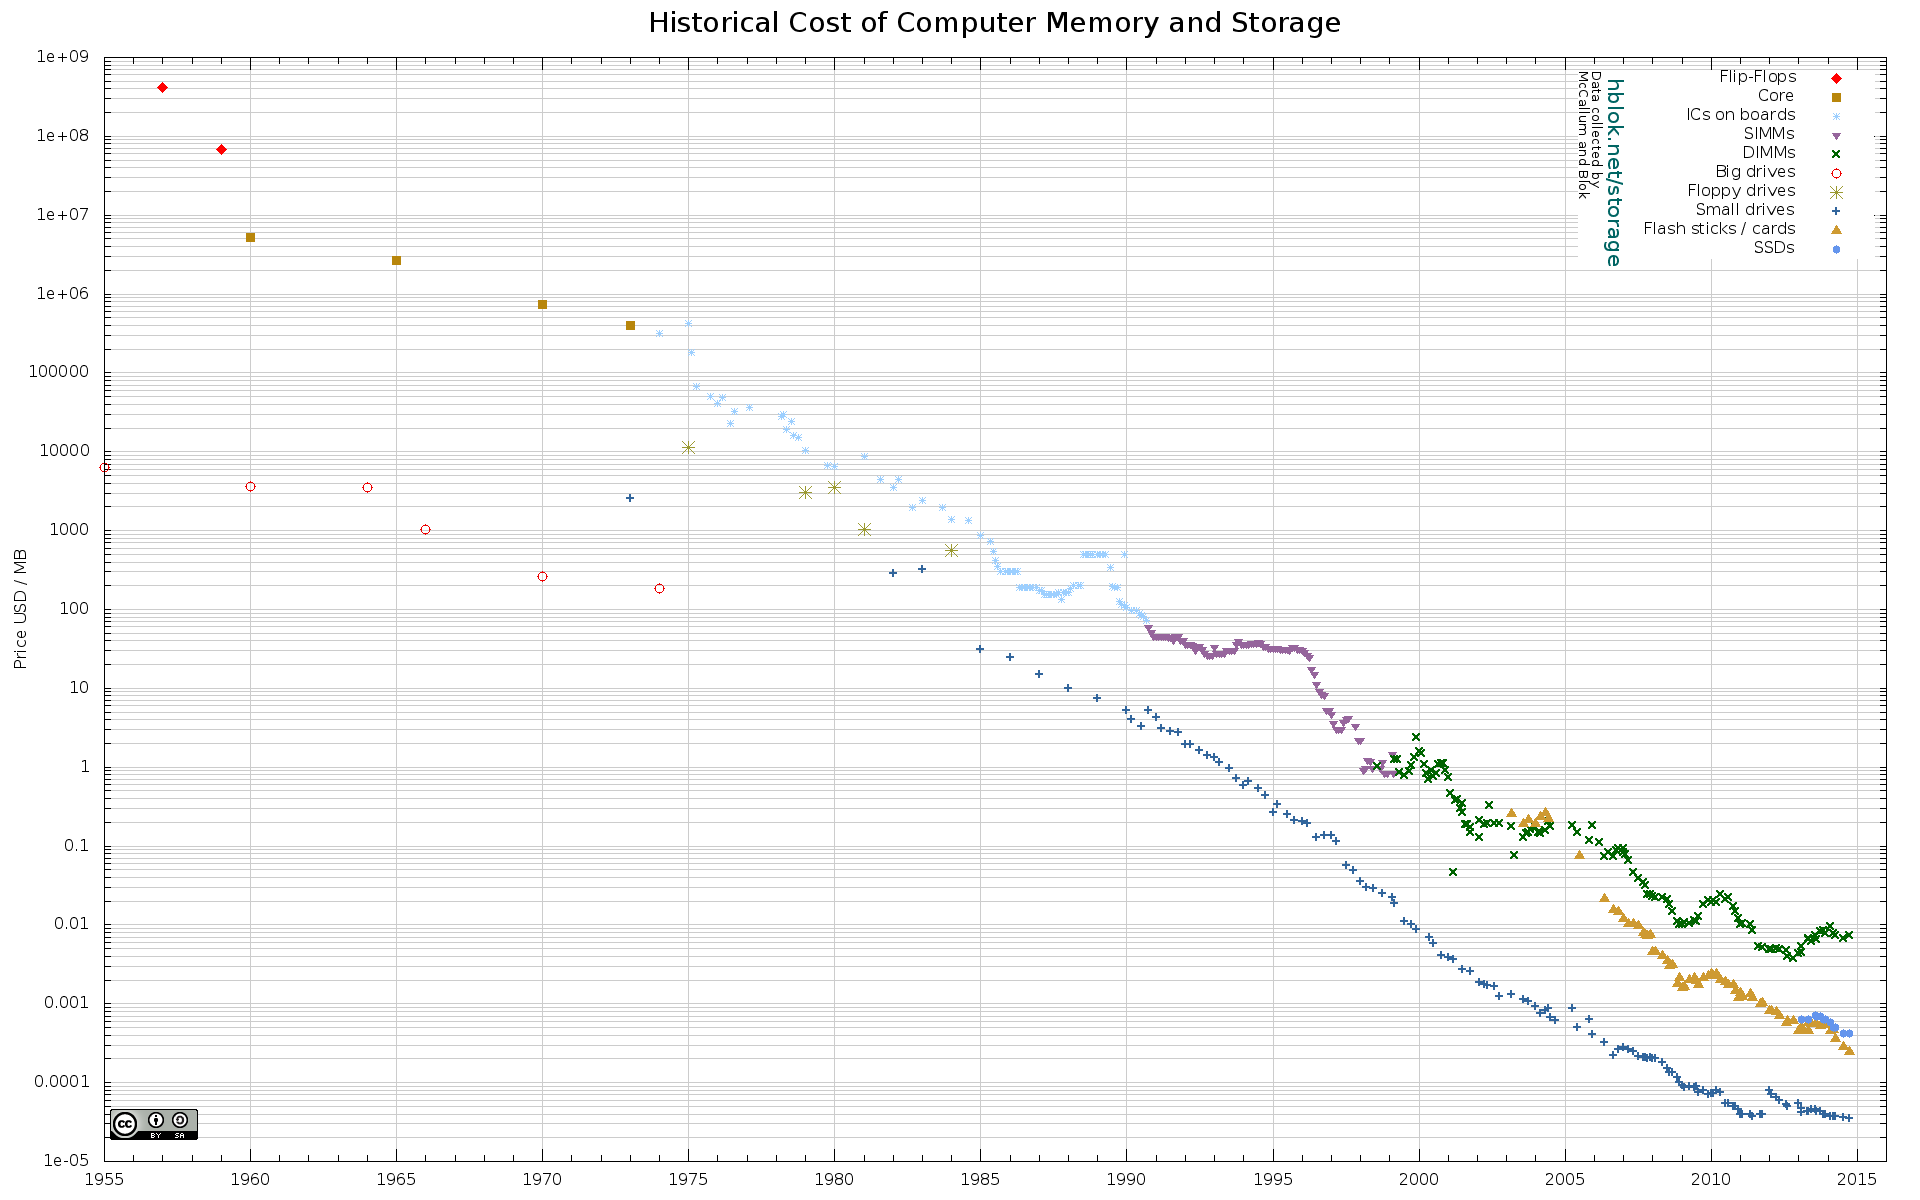
\includegraphics[width=\textwidth]{figures/exampleFigure.png} % Adjust width and file path as needed.
	\caption[Figure title for the Table of Contents]{ 
    Figure title for the main text. % By default, this should be identical to the figure title used in the Table of Contents.
    \textmd{Type a longer subtitle or caption here, optionally, which appears unbolded in the main text.}
    }
	\label{figurelabel} % Refer to this figure in the main text by typing \ref{figurelabel}. Be sure to give each figure a unique and sensible label.
\end{figure}



Lorem ipsum dolor sit amet, consectetur adipiscing elit, sed do eiusmod tempor incididunt ut labore et dolore magna aliqua. Ut enim ad minim veniam, quis nostrud exercitation ullamco laboris nisi ut aliquip ex ea commodo consequat \cite{ref1}. Duis aute irure dolor in reprehenderit in voluptate velit esse cillum dolore eu fugiat nulla pariatur \cite{ref2}. Excepteur sint occaecat cupidatat non proident, sunt in culpa qui officia deserunt mollit anim id est laborum \cite{ref3}.

Lorem ipsum dolor sit amet, consectetur adipiscing elit, sed do eiusmod tempor incididunt ut labore et dolore magna aliqua. Ut enim ad minim veniam, quis nostrud exercitation ullamco laboris nisi ut aliquip ex ea commodo consequat \cite{ref1}. Duis aute irure dolor in reprehenderit in voluptate velit esse cillum dolore eu fugiat nulla pariatur \cite{ref2}. Excepteur sint occaecat cupidatat non proident, sunt in culpa qui officia deserunt mollit anim id est laborum.

Lorem ipsum dolor sit amet, consectetur adipiscing elit, sed do eiusmod tempor incididunt ut labore et dolore magna aliqua. Ut enim ad minim veniam, quis nostrud exercitation ullamco laboris nisi ut aliquip ex ea commodo consequat \cite{ref1}. Duis aute irure dolor in reprehenderit in voluptate velit esse cillum dolore eu fugiat nulla pariatur \cite{ref2}. Excepteur sint occaecat cupidatat non proident, sunt in culpa qui officia deserunt mollit anim id est laborum.

Lorem ipsum dolor sit amet, consectetur adipiscing elit, sed do eiusmod tempor incididunt ut labore et dolore magna aliqua. Ut enim ad minim veniam, quis nostrud exercitation ullamco laboris nisi ut aliquip ex ea commodo consequat \cite{ref1}. Duis aute irure dolor in reprehenderit in voluptate velit esse cillum dolore eu fugiat nulla pariatur \cite{ref2}. Excepteur sint occaecat cupidatat non proident, sunt in culpa qui officia deserunt mollit anim id est laborum.

Lorem ipsum dolor sit amet, consectetur adipiscing elit, sed do eiusmod tempor incididunt ut labore et dolore magna aliqua. Ut enim ad minim veniam, quis nostrud exercitation ullamco laboris nisi ut aliquip ex ea commodo consequat \cite{ref1}. Duis aute irure dolor in reprehenderit in voluptate velit esse cillum dolore eu fugiat nulla pariatur \cite{ref2}. Excepteur sint occaecat cupidatat non proident, sunt in culpa qui officia deserunt mollit anim id est laborum.

Lorem ipsum dolor sit amet, consectetur adipiscing elit, sed do eiusmod tempor incididunt ut labore et dolore magna aliqua. Ut enim ad minim veniam, quis nostrud exercitation ullamco laboris nisi ut aliquip ex ea commodo consequat \cite{ref1}. Duis aute irure dolor in reprehenderit in voluptate velit esse cillum dolore eu fugiat nulla pariatur \cite{ref2}. Excepteur sint occaecat cupidatat non proident, sunt in culpa qui officia deserunt mollit anim id est laborum.

% This is a table
%If you are having issues with \midline use \hline insteadn and remove booktabs package from thesis.tex

\begin{table}
\caption{This is an example Table.}
\begin{center}
\begin{tabular}{ccc}
x & f(x) & g(x) \\
%\hline
\midrule
1 & 6 & 4  \\
2 & 6 & 3  \\
3 & 6 & 2  \\
4 & 6 & 2  \\
\label{Table in Chapter 1}
\end{tabular}
\end{center}
\end{table}



%%%%%%%%%%%%%%%%
% Chapter 2
%%%%%%%%%%%%%%%%

\chapter{Title of Chapter Two}

Lorem ipsum dolor sit amet, consectetur adipiscing elit, sed do eiusmod tempor incididunt ut labore et dolore magna aliqua. Etiam sit amet nisl purus in mollis nunc sed id. Arcu ac tortor dignissim convallis aenean et tortor at risus. Facilisi morbi tempus iaculis urna id volutpat lacus laoreet. Quis commodo odio aenean sed adipiscing. Elementum nibh tellus molestie nunc non blandit. Elit ut aliquam purus sit amet luctus venenatis. Sollicitudin ac orci phasellus egestas tellus rutrum. Sit amet nulla facilisi morbi tempus iaculis urna id volutpat. Nibh cras pulvinar mattis nunc sed blandit libero volutpat. Rhoncus urna neque viverra justo. Amet tellus cras adipiscing enim eu turpis egestas. Leo vel orci porta non pulvinar neque laoreet suspendisse.

\section{Important Dissertation Research}

Vel fringilla est ullamcorper eget nulla facilisi etiam. Cras semper auctor neque vitae tempus quam pellentesque nec nam. Phasellus vestibulum lorem sed risus ultricies tristique nulla aliquet. Rhoncus est pellentesque elit ullamcorper dignissim cras tincidunt lobortis feugiat. Eu ultrices vitae auctor eu augue ut lectus arcu. Mi sit amet mauris commodo quis imperdiet massa tincidunt nunc. Elit eget gravida cum sociis natoque penatibus et. Aliquet porttitor lacus luctus accumsan. In hac habitasse platea dictumst vestibulum. Viverra vitae congue eu consequat ac. Nisi quis eleifend quam adipiscing vitae proin sagittis nisl rhoncus. Risus pretium quam vulputate dignissim suspendisse in.

\section{More Important Dissertation Research}

Nascetur ridiculus mus mauris vitae ultricies leo integer malesuada. Duis at tellus at urna condimentum. Maecenas sed enim ut sem. Mattis vulputate enim nulla aliquet porttitor lacus. Imperdiet proin fermentum leo vel orci porta non pulvinar neque. Non pulvinar neque laoreet suspendisse interdum. Arcu risus quis varius quam. Suscipit adipiscing bibendum est ultricies integer quis auctor. Amet aliquam id diam maecenas. Mauris nunc congue nisi vitae. Mus mauris vitae ultricies leo integer malesuada nunc. Rhoncus est pellentesque elit ullamcorper dignissim cras tincidunt lobortis. Fringilla ut morbi tincidunt augue interdum. Dui vivamus arcu felis bibendum ut tristique et egestas quis. Non enim praesent elementum facilisis leo vel fringilla est ullamcorper. Elit at imperdiet dui accumsan. Scelerisque felis imperdiet proin fermentum leo vel orci porta. Neque viverra justo nec ultrices dui sapien eget mi.

\subsection{Explanation of Important Dissertation Research}

Varius vel pharetra vel turpis. In cursus turpis massa tincidunt dui ut ornare lectus sit. Risus pretium quam vulputate dignissim suspendisse in. Dolor sit amet consectetur adipiscing elit duis tristique sollicitudin nibh. In est ante in nibh mauris. Pellentesque adipiscing commodo elit at imperdiet. Dapibus ultrices in iaculis nunc. Nulla facilisi nullam vehicula ipsum a arcu cursus. Malesuada fames ac turpis egestas sed tempus urna et pharetra. Donec enim diam vulputate ut pharetra sit. Quisque sagittis purus sit amet volutpat consequat.








%%%%%%%%%%%%%%%%
% Chapter 3
%%%%%%%%%%%%%%%%

\chapter{Title of Chapter Three}

Lorem ipsum dolor sit amet, consectetur adipiscing elit, sed do eiusmod tempor incididunt ut labore et dolore magna aliqua. Ut enim ad minim veniam, quis nostrud exercitation ullamco laboris nisi ut aliquip ex ea commodo consequat. Duis aute irure dolor in reprehenderit in voluptate velit esse cillum dolore eu fugiat nulla pariatur. Excepteur sint occaecat cupidatat non proident, sunt in culpa qui officia deserunt mollit anim id est laborum.


%%%%%%%%%%%%%%%%
% Chapter 4
%%%%%%%%%%%%%%%%

\chapter{Title of Chapter Four}

The final chapter! If you need more chapters, simply create a new file called \url{chapter5.tex} and include it in the main \url{thesis.tex} file in the same way that the other chapters were included.





%%%%%%%%%%%%%%%%
% Conclusion
%%%%%%%%%%%%%%%%


\clearpage
\phantomsection
\addcontentsline{toc}{chapter}{Conclusion or Epilogue}

\begin{center}
\pagebreak
\vspace*{5\baselineskip}
\textbf{\large Conclusion or Epilogue}
\end{center}


\begin{flushleft}
\hspace{10mm}Use this page for your epilogue or conclusion if applicable; please use only one of the titles for this page. Otherwise, you may delete it.
Use this page for your epilogue or conclusion if applicable; please use only one of the titles for this page. Otherwise, you may delete it.
Use this page for your epilogue or conclusion if applicable; please use only one of the titles for this page. Otherwise, you may delete it.
Use this page for your epilogue or conclusion if applicable; please use only one of the titles for this page. Otherwise, you may delete it.
Use this page for your epilogue or conclusion if applicable; please use only one of the titles for this page. Otherwise, you may delete it.
Use this page for your epilogue or conclusion if applicable; please use only one of the titles for this page. Otherwise, you may delete it.
Use this page for your epilogue or conclusion if applicable; please use only one of the titles for this page. Otherwise, you may delete it.
Use this page for your epilogue or conclusion if applicable; please use only one of the titles for this page. Otherwise, you may delete it.
Use this page for your epilogue or conclusion if applicable; please use only one of the titles for this page. Otherwise, you may delete it.Use this page for your epilogue or conclusion if applicable; please use only one of the titles for this page. Otherwise, you may delete it.Use this page for your epilogue or conclusion if applicable; please use only one of the titles for this page. Otherwise, you may delete it.
Use this page for your epilogue or conclusion if applicable; please use only one of the titles for this page. Otherwise, you may delete it.Use this page for your epilogue or conclusion if applicable; please use only one of the titles for this page. Otherwise, you may delete it.
Use this page for your epilogue or conclusion if applicable; please use only one of the titles for this page. Otherwise, you may delete it.
Use this page for your epilogue or conclusion if applicable; please use only one of the titles for this page. Otherwise, you may delete it.
Use this page for your epilogue or conclusion if applicable; please use only one of the titles for this page. Otherwise, you may delete it.
Use this page for your epilogue or conclusion if applicable; please use only one of the titles for this page. Otherwise, you may delete it.
Use this page for your epilogue or conclusion if applicable; please use only one of the titles for this page. Otherwise, you may delete it.
Use this page for your epilogue or conclusion if applicable; please use only one of the titles for this page. Otherwise, you may delete it.
Use this page for your epilogue or conclusion if applicable; please use only one of the titles for this page. Otherwise, you may delete it.
Use this page for your epilogue or conclusion if applicable; please use only one of the titles for this page. Otherwise, you may delete it.
Use this page for your epilogue or conclusion if applicable; please use only one of the titles for this page. Otherwise, you may delete it.
Use this page for your epilogue or conclusion if applicable; please use only one of the titles for this page. Otherwise, you may delete it.Use this page for your epilogue or conclusion if applicable; please use only one of the titles for this page. Otherwise, you may delete it.Use this page for your epilogue or conclusion if applicable; please use only one of the titles for this page. Otherwise, you may delete it.
Use this page for your epilogue or conclusion if applicable; please use only one of the titles for this page. Otherwise, you may delete it.Use this page for your epilogue or conclusion if applicable; please use only one of the titles for this page. Otherwise, you may delete it.
Use this page for your epilogue or conclusion if applicable; please use only one of the titles for this page. Otherwise, you may delete it.
Use this page for your epilogue or conclusion if applicable; please use only one of the titles for this page. Otherwise, you may delete it.
Use this page for your epilogue or conclusion if applicable; please use only one of the titles for this page. Otherwise, you may delete it.
Use this page for your epilogue or conclusion if applicable; please use only one of the titles for this page. Otherwise, you may delete it.
Use this page for your epilogue or conclusion if applicable; please use only one of the titles for this page. Otherwise, you may delete it.
Use this page for your epilogue or conclusion if applicable; please use only one of the titles for this page. Otherwise, you may delete it.
Use this page for your epilogue or conclusion if applicable; please use only one of the titles for this page. Otherwise, you may delete it.
Use this page for your epilogue or conclusion if applicable; please use only one of the titles for this page. Otherwise, you may delete it.
Use this page for your epilogue or conclusion if applicable; please use only one of the titles for this page. Otherwise, you may delete it.
Use this page for your epilogue or conclusion if applicable; please use only one of the titles for this page. Otherwise, you may delete it.Use this page for your epilogue or conclusion if applicable; please use only one of the titles for this page. Otherwise, you may delete it.Use this page for your epilogue or conclusion if applicable; please use only one of the titles for this page. Otherwise, you may delete it.
Use this page for your epilogue or conclusion if applicable; please use only one of the titles for this page. Otherwise, you may delete it.Use this page for your epilogue or conclusion if applicable; please use only one of the titles for this page. Otherwise, you may delete it.
Use this page for your epilogue or conclusion if applicable; please use only one of the titles for this page. Otherwise, you may delete it.
Use this page for your epilogue or conclusion if applicable; please use only one of the titles for this page. Otherwise, you may delete it.
Use this page for your epilogue or conclusion if applicable; please use only one of the titles for this page. Otherwise, you may delete it.
Use this page for your epilogue or conclusion if applicable; please use only one of the titles for this page. Otherwise, you may delete it.
Use this page for your epilogue or conclusion if applicable; please use only one of the titles for this page. Otherwise, you may delete it.
Use this page for your epilogue or conclusion if applicable; please use only one of the titles for this page. Otherwise, you may delete it.
Use this page for your epilogue or conclusion if applicable; please use only one of the titles for this page. Otherwise, you may delete it.
Use this page for your epilogue or conclusion if applicable; please use only one of the titles for this page. Otherwise, you may delete it.
Use this page for your epilogue or conclusion if applicable; please use only one of the titles for this page. Otherwise, you may delete it.
Use this page for your epilogue or conclusion if applicable; please use only one of the titles for this page. Otherwise, you may delete it.Use this page for your epilogue or conclusion if applicable; please use only one of the titles for this page. Otherwise, you may delete it.Use this page for your epilogue or conclusion if applicable; please use only one of the titles for this page. Otherwise, you may delete it.
Use this page for your epilogue or conclusion if applicable; please use only one of the titles for this page. Otherwise, you may delete it.Use this page for your epilogue or conclusion if applicable; please use only one of the titles for this page. Otherwise, you may delete it.
Use this page for your epilogue or conclusion if applicable; please use only one of the titles for this page. Otherwise, you may delete it.
Use this page for your epilogue or conclusion if applicable; please use only one of the titles for this page. Otherwise, you may delete it.
Use this page for your epilogue or conclusion if applicable; please use only one of the titles for this page. Otherwise, you may delete it.
Use this page for your epilogue or conclusion if applicable; please use only one of the titles for this page. Otherwise, you may delete it.
Use this page for your epilogue or conclusion if applicable; please use only one of the titles for this page. Otherwise, you may delete it.
Use this page for your epilogue or conclusion if applicable; please use only one of the titles for this page. Otherwise, you may delete it.
Use this page for your epilogue or conclusion if applicable; please use only one of the titles for this page. Otherwise, you may delete it.
Use this page for your epilogue or conclusion if applicable; please use only one of the titles for this page. Otherwise, you may delete it.
Use this page for your epilogue or conclusion if applicable; please use only one of the titles for this page. Otherwise, you may delete it.
Use this page for your epilogue or conclusion if applicable; please use only one of the titles for this page. Otherwise, you may delete it.Use this page for your epilogue or conclusion if applicable; please use only one of the titles for this page. Otherwise, you may delete it.Use this page for your epilogue or conclusion if applicable; please use only one of the titles for this page. Otherwise, you may delete it.
Use this page for your epilogue or conclusion if applicable; please use only one of the titles for this page. Otherwise, you may delete it.Use this page for your epilogue or conclusion if applicable; please use only one of the titles for this page. Otherwise, you may delete it.
Use this page for your epilogue or conclusion if applicable; please use only one of the titles for this page. Otherwise, you may delete it.
\end{flushleft}


%\pagenumbering{gobble}  %remove page number on summary page





%%%%%%%%%%%%%%%%
% References
%%%%%%%%%%%%%%%%
\clearpage
\phantomsection 
\titleformat{\chapter}[display]
{\normalfont\bfseries\filcenter}{}{0pt}{\large\bfseries\filcenter{#1}}  % Reset title format for Reference section. (It is different from Chapter titles)
\titlespacing*{\chapter}
  {0pt}{0pt}{30pt}

\begin{singlespace}  % use single-line spacing for multi-line text within a single reference
	\setlength\bibitemsep{\baselineskip}  %manually set separataion betwen items in bibliography to double space
	\addcontentsline{toc}{chapter}{References}  %add References section to Table of Contents
	\printbibliography[title={References}]
\end{singlespace}



%%%%%%%%%%%%%%%%
% Appendices
%%%%%%%%%%%%%%%%

%Readjust Title format for Appendicies
\titleformat{\chapter}[display]
{\normalfont\bfseries\filcenter}{}{0pt}{\large\chaptertitlename\ \large\thechapter : \large\bfseries\filcenter{#1}}  
\titlespacing*{\chapter}
  {0pt}{0pt}{30pt}	%controls vertical margins on title
  
% Adjust section title formatting
\titleformat{\section}{\normalfont\bfseries}{\thesection}{1em}{#1}

% Adjust subsection title formatting
\titleformat{\subsection}{\normalfont}{\thesubsection}{0em}{\hspace{1em}#1}

\begin{appendices}

%Some Table of Contents entry formatting
\addtocontents{toc}{\protect\renewcommand{\protect\cftchappresnum}{\appendixname\space}}
\addtocontents{toc}{\protect\renewcommand{\protect\cftchapnumwidth}{6em}}

%Begin individual appendices, separated as chapters

\chapter{ Experimental Equipment}
Lorem ipsum dolor sit amet, consectetur adipiscing elit, sed do eiusmod tempor incididunt ut labore et dolore magna aliqua. Ut enim ad minim veniam, quis nostrud exercitation ullamco laboris nisi ut aliquip ex ea commodo consequat. Duis aute irure dolor in reprehenderit in voluptate velit esse cillum dolore eu fugiat nulla pariatur. Excepteur sint occaecat cupidatat non proident, sunt in culpa qui officia deserunt mollit anim id est laborum.

\chapter{Data Processing}
Lorem ipsum dolor sit amet, consectetur adipiscing elit, sed do eiusmod tempor incididunt ut labore et dolore magna aliqua. Ut enim ad minim veniam, quis nostrud exercitation ullamco laboris nisi ut aliquip ex ea commodo consequat. Duis aute irure dolor in reprehenderit in voluptate velit esse cillum dolore eu fugiat nulla pariatur. Excepteur sint occaecat cupidatat non proident, sunt in culpa qui officia deserunt mollit anim id est laborum.

\end{appendices}

\end{document} 
